\documentclass{article}
\usepackage[numbers]{natbib}
\usepackage{blindtext}
\usepackage{titlesec}
\usepackage{amsmath}
\usepackage{amssymb}
\usepackage{amsthm}
\usepackage{hyperref}
\usepackage{graphicx}
\newtheorem{definition}{Definition}
\newtheorem{theorem}{Theorem}
\hypersetup{
    colorlinks=true,
    linkcolor=blue,
    urlcolor=blue,
}
\bibliographystyle{unsrtnat}
\usepackage[utf8]{inputenc}

\title{Theory Group Seminar Notes}
\author{Rishit Dagli}
\date{October 2022}

\begin{document}

\maketitle

\tableofcontents
\clearpage

\addcontentsline{toc}{section}{Introduction}
\section*{Introduction}

These are my notes for the seminars that happen in the \href{https://www.cs.toronto.edu/theory/}{Theory Group} at The University of Toronto. Many thanks to \href{http://www.cs.toronto.edu/~bor/}{Professor Allan Borodin} for allowing me to attend the Theory Group seminars and helping out.\\

A PDF of these notes is available at \url{https://rishit-dagli.github.io/cs-theory-notes/main.pdf}. An online version of these notes are available at \url{https://rishit-dagli.github.io/cs-theory-notes}.\\

The Theory Group focuses on theory of computation. The group is interested in using mathematical techniques to understand the nature of computation and to design and analyze algorithms for important and fundamental problems.\\

The members of the theory group are all interested, in one way or another, in the limitations of computation: What problems are not feasible to solve on a computer? How can the infeasibility of a problem be used to rigorously construct secure cryptographic protocols? What problems cannot be solved faster using more machines? What are the limits to how fast a particular problem can be solved or how much space is needed to solve it? How do randomness, parallelism, the operations that are allowed, and the need for fault tolerance or security affect this?

\newpage

\section{Lower Bounds for Locally Decodable Codes from Semirandom CSP Refutation}

7th October 2022\\

\noindent The related paper: Combinatorial lower bounds for 3-query LDCs by \citet{Alrabiah2022-ds}. Seminar by \href{https://www.cs.cmu.edu/~pmanohar/}{Peter Manohar}. \cite{https://doi.org/10.48550/arxiv.1911.10698} \cite{https://doi.org/10.48550/arxiv.2109.04415}

\subsection{Abstract}

A code $C$ is a q-locally decodable code (q-LDC) if one can recover any chosen bit $b_i$ of the $k$-bit message b with good confidence by randomly querying the $n$-bit encoding x on at most $q$ coordinates. Existing constructions of $2$-LDCs achieve blocklength $n = exp(O(k))$, and lower bounds show that this is in fact tight. However, when $q = 3$, far less is known: the best constructions have $n = subexp(k)$, while the best known lower bounds, that have stood for nearly two decades, only show a quadratic lower bound of $n \geq \Omega(k^2)$ on the blocklength.\\

\noindent In this talk, we will survey a new approach to prove lower bounds for LDCs using recent advances in refuting semirandom instances of constraint satisfaction problems. These new tools yield, in the $3$-query case, a near-cubic lower bound of $n \geq \tilde{\Omega}(k^3)$, improving on prior work by a polynomial factor in $k$.

\subsection{Locally Decodable Codes}

Take codes $b \in {0,1}^k \rightarrow x \in {0,1}^n$

\noindent Codes $x$ are read by the decoder, $i \in [k]$, $\hat{b_i} \in {0,1}$

\begin{definition}
$C$ is a $(q, \delta, \epsilon)$-locally decodable if for any $x$ with $\bigtriangleup(x, Enc(b)) \leq \delta n$, $Dec^x(i) = b_i$ w.p. $\geq \frac{1}{2} + \epsilon$ for any $i$.
\end{definition}

\noindent Ask the question, what is the best possible rate for a $q$-LDC given a $q$?

\begin{center}
\begin{tabular}{ |c|c|c| } 
 \hline
 $q$ & Lower Bound & Upper Bound \\
 \hline
 2 & $2^{\Omega(k)} \leq n$ & $n \leq 2^k$ \\ 
 3 & $k^2 \leq n$ & $n \leq exp(k^{o(1)})$ \\
 $O(1)$, even & $k^{\frac{q}{q+1}} \leq n$ & $n \leq exp(k^{o(1)})$ \\ 
 $O(1)$, odd & $k^{\frac{q+1}{q-1}} \leq n$ & $n \leq exp(k^{o(1)})$ \\ 
 \hline
\end{tabular}
\end{center}

\noindent Focus on the case $q=3$, we have gotten better bounds:

\begin{equation}
k \leq n \leq 2^k
\end{equation}

\begin{equation*}
k^2 \leq n \leq exp(exp(\sqrt{\log k \log \log k}))
\end{equation*}

\noindent In \cite{Alrabiah2022-ds}, they show that a better minimum bound can be found than these existing ones for $q=3$:

\begin{equation}
k^3 \leq n
\end{equation}

\noindent The main result is that:

\begin{theorem}
Let $C$ be a $(3, \delta, \epsilon)$-locally decodable codes. Then $n \geq \tilde{\Omega}_{\delta, \epsilon}(k^3)$.
\end{theorem}

\noindent Semi-random CSP refutation comes to our aid to prove this! The intuitive way to put this theorem is that $q$-LDC lower bound is same as refuting "LDC" $q$-XOR.

\subsection{How to prove the Theorem}

The idea:

\begin{itemize}
    \item $q$-LDC lower bound is same as refuting "LDC" $q$-XOR \phantomsection\label{proofp1}
        \begin{itemize}
            \item CSP Refutation
        \end{itemize}
    \item Proof of existing $q$-LDC lower bound for $q$ even
    \item Proof sketch of $k^3$ lower bound
\end{itemize}

\subsection{Normally Decodable Codes}

We can see that the decoder we have can arbitrary but WLOG we can assume there are $q$-unif hypergraphs ${H_1, H_2, \cdots H_k}$ where every $H_i$ is such that:

\begin{equation*}
H_i \subseteq {[n] \choose q}
\end{equation*}

\noindent We can also see that:

\noindent Each $H_i$ is a matching such that $|H_i| \geq \delta n$

\noindent and, $Dec(i)$ picks $C \leftarrow H_i$ and outputs $\sum_{j \in C} x_j$\\

\noindent One such example is the Hadmard code:

\begin{equation}
b \in {0,1}^k \mapsto f = (\langle b, v \rangle)_{v \in {0,1}}^k
\end{equation}

\begin{equation*}
b_i = f(e_i) = f(v) + f(v+e_i)
\end{equation*}

\noindent Can think of this as $v$ and $v+e_i$ are connected.\\

\noindent Matching vector codes are $\approx \mathbb{Z} _{m}^{h}$

\subsection{Proof: Going from LDC to XOR}

We suppose that our code is linear and that there exists $q$-unif hypergraphs ${H_1, H_2, \cdots H_k}$.\\

\noindent We also know that:

Each $H_i$ is a matching such that $|H_i| \geq \delta n$

and, $Dec(i)$ picks $C \leftarrow H_i$ and outputs $\sum_{j \in C} x_j$\\

\noindent So, we start by considering a $q$-XOR instance $\psi_b$:

\begin{equation*}
\begin{split}
    \textit{Vars: } & \{x_j\}_{j \in [n]}\\
    \textit{Over Equations: } & \sum_{j \in C} x_j = b_i, \forall i \in [k], C \in H_i
\end{split}
\end{equation*}

\noindent We can write down the maximum fraction of satisfiable constraints: $val(\psi_b) = 1$ for any $b \in {0,1}^k$.\\

\noindent It is sufficient now if we can argue that $\psi_b$ is unsat with high probability for some random $b$ when $n \ll k^{\frac{q}{q-2}}$.\\

\noindent Now we need to refute XOR, there are many ways to argue unsatisfiability of an XOR instance. One reason why we can not use probablistic approaches here is that $\psi_b$ only has $k$ bits of randomness.\\

\noindent One way we can have some success here is to use a refutation algorithm

\begin{equation*}
\psi \rightarrow A \rightarrow algval(\psi)
\end{equation*}

\noindent With this the guarantee then would be $val(\psi) \leq algval(\psi)$ which is similar to saying that if $algval(\psi) < 1$ then $A$ refutes $\psi$. The ideal goal would be to refute random $\psi$ with $m$ constraints with high probability\\

\noindent However, we take a look at semi-random XOR. Our refutation algorithm and the guarantee will still be the same:

\begin{equation*}
\psi \rightarrow A \rightarrow algval(\psi)
\end{equation*}

\noindent with the guarantee that $val(\psi) \leq algval(\psi)$.\\

\noindent So, now we generate semi-random $\psi w/ m$ constraints:

\begin{itemize}
    \item The worst case would be random $q$-unif hypergraph
    \item Random RHS $b_c$ for each $C \in H$
\end{itemize}

\noindent The equation we have is:

\begin{equation}
    \sum_{j \in C} x_j = b_c
\end{equation}

\noindent And we also already know that 

\begin{equation*}
    \psi_b \textit{ is } \sum_{j \in C}
\end{equation*}

\noindent And, $xj = b_i, i \in [k], C \in H_i$.

\noindent $\psi_b$ is almost semi-random.\\

\noindent Thus, we have shown \ref{proofp1}{ Part 1 of Proof}.

\subsection{Proof: Existing $q$-LDC lower bound for $q$ even}

$q$-LDC XOR instance $\psi_b$ is encoded by:

\begin{itemize}
    \item $q$-uniform hypergraph matchings $\{ H_1 \cdots H_k \}$
    \item right-hand sides are random $b_i \in \{ \pm 1 \}$
    \item We have constraints $\displaystyle\prod_{j \in C} x_j=b_i$ for all $i$ and $C \in H_i$
\end{itemize}

\noindent We now have a goal to argue that $\psi_b$ unsat with high probability for random when $b$ when $n \ll k^{q/(q-2)}$\\

\noindent frac. constraints satisfied by $x \in \{ \pm 1 \}^n$ is $\frac{1}{2} + \frac{f(x)}{2}$.\\

\noindent Here $f(x)$ is:

\begin{equation}\label{eq:5}
f(x) = \frac{1}{m} \sum_{i} b_i \sum_{C \in H_i} \prod_{j \in C} x_j
\end{equation}
\begin{equation*}
m = k \cdot \delta n
\end{equation*}

\noindent This makes our goal to be to certify with high probability that:

\begin{equation}\label{eq:6}
\max_{x \in \{ \pm 1 \}^n} f(x) < 1 \textit{ when } n \ll k^{\frac{q}{q-2}}
\end{equation}

\noindent We will now try to refute $\psi_b$. With Equation \ref{eq:5} and Equation \ref{eq:6} to refute $\psi_b$ is like showing:

\begin{equation}
\textit{w.h.p. } \max_{x \in \{ \pm 1 \}^n} f(x) < 1 \textit{ where } f(x) = \frac{1}{m} \sum_{i} b_i \sum_{C \in H_i} \prod_{j \in C} x_j
\end{equation}

\noindent $\textit{ when } n \ll k^{\frac{q}{q-2}}$.\\

\noindent The idea is to design a matrix $A \in \mathbb{R}^{N \times N}$ so that:

\begin{equation*}
f(x) \leq ||A||_{\infty \to 1} = \max_{z,w \in \{ \pm 1 \}^N} z^TAw
\end{equation*}

\noindent As shown by \citet{https://doi.org/10.48550/arxiv.1904.03858} the matrix $A$ can be indexed by

\begin{equation*}
S \in {[n] \choose l}
\end{equation*}

\noindent Assign $x \mapsto y$ such that $y^TAy \propto f(x)$

\noindent and $y_s := \displaystyle\prod_{j \in S} x_j$ which is simply the tensor product.\\\

\noindent We need to now be able to answer how to set $A(S,T)$

\begin{equation}
y^TAy = \sum_{S,T} y_Sy_TA(S,T) = \sum_{S,T} A(S,T) \displaystyle\prod_{j \in S \oplus T} x_j
\end{equation}

\noindent Which shows that we are actually using symmetric difference here.\\

\noindent We say that if $S \oplus T = C \in h_i$ then $\displaystyle\prod_{j \in S \oplus T} x_j = b_i$

\noindent $\implies A(S,T) = b_i$ if $S \oplus T = C \in H_i$\\

\begin{equation}
y^TAy = \sum_{i=1}^k b_i \sum_{C \in h_i} \sum_{S \oplus t = C} \displaystyle\prod_{j \in C}x_j = Dmf(x)
\end{equation}

\noindent Here $D =$ number of $S,T$ where $S \oplus T = C$.\\

\noindent Simplifying an earlier statement we can also say from here that: $A_C(S,T) = 1$ if $S \oplus T = C$.\\

\noindent For which $A_i = \sum_{C \in h_i} A_C$ and $A = \sum_{i=1}^k b_i A_i$\\

\noindent Set $y_S := \displaystyle\prod_{j \in S} x_j$\\

\noindent $y^TAy = Dmf(x) \implies Dmf(x) \leq ||A||_{\infty \to 1}$\\

\noindent Note that the way we defined $D$ here it only depends on $|C| = q$, we can say:

\begin{equation*}
D = {q \choose \frac{q}{2}} {n-q \choose l - \frac{q}{2}}
\end{equation*}

\noindent Also we know $A_c \in \mathbb{R}^{N \times N}$ and $N = {n \choose l}$.\\

\noindent We have already proven that $||A||_{\infty \to 1} \geq Dm \max_{x}f(x) \geq Dm \geq D \delta nk$\\

\noindent It is also interesting to note that $||A||_{\infty \to 1} \leq N ||A||_2$ and we still need to be able to show that with high probability that $||A||_{\infty \to 1}$ is not too large.\\

\noindent Matrix Bernstein: with high probability over $b_i$, $||A||_2 \leq \triangle \sqrt{kl}$ where $\triangle$ is the maximum number of 1's in a row in any $A_i$.\\

\noindent Expected number of 1's per row is $\delta n \frac{D}{N} \sim n (\frac{l}{n})^{q/2}$.\\

\noindent We can optimistically suppose that $\triangle \sim n (\frac{l}{n})^{q/2}$ however this also needs $l \geq n^{1-2/q}$.\\

\noindent Then $D \cdot \delta n k \leq ||A||_{\infty \to  1} \leq N \triangle \sqrt{kl}$\\

\noindent $\implies k \leq l$ since $\triangle \sim \delta n \frac{D}{N}$\\

\noindent Now take $l=n^{1-2/q} \implies k^{q/(q-2)} \leq n$\\

\noindent So, $\triangle =\frac{2l}{q}$\\

\noindent Because $H_i$ are matchings, a random row will have only $\approx \frac{\delta n D}{N}$ 1's.\\

\noindent The idea now is to prune off all the bad rows or columns in A to get B such that:

\begin{equation*}
||A||_{\infty \to 1} \leq ||B||_{\infty \to 1} +o(N)
\end{equation*}

\noindent And, $\triangle_B \sim \delta n (\frac{l}{n})^{q/2}$\\

\noindent And now we can just use $B$ instead which will prove $q$-LDC lower bound for $q$ even.

\subsection{Proof: $k^3$ lower bound}

Recall, $q$-LDC XOR instance $\psi_b$ is encoded by:

\begin{itemize}
    \item $q$-uniform hypergraph matchings $\{ H_1 \cdots H_k \}$
    \item right-hand sides are random $b_i \in \{ \pm 1 \}$
    \item We have constraints $\displaystyle\prod_{j \in C} x_j=b_i$ for all $i$ and $C \in H_i$
\end{itemize}

\noindent The goal is argue that $\psi_b$ is unsatisfiable with high probability for random $b$. And the idea is to design a matrix $A \in \mathbb{R}^{N \times N}$ so that:

\begin{equation*}
f(x) \leq ||A||_{\infty \to 1} = \max_{z, w \in \{ \pm 1 \}^N z^TAw}
\end{equation*}

\noindent The previous approach fails because the $A$ from before requires $q$ to be even.\\

\noindent One attempt is to represent rows as $|S|=l$ and columns as $|T|=l+1$. However this will only get us to $k \leq \sqrt{n}$.\\

\noindent We need to derive more constraints, using $C_i \oplus C_j$ get us to $nk$ constraints so each $n_j$ is in $\approx k$ constraints $\implies$ new $nk^2$ constraints. \\

\noindent The matrix $A$ is indexed by $S$, $A(S,T)=b_ib_j$. The calculation is now:

\begin{equation*}
nk^2D \leq ||A||_{\infty \to 1} \leq N \triangle \sqrt{kl}
\end{equation*}

\noindent An optimist approach is $\triangle \sim Nk\frac{D}{N} = nk(\frac{l}{n})^2$\\

\noindent $\implies l \geq \sqrt{\frac{n}{k}}$\\

\noindent $\implies k \leq n \implies k^3 \leq n$\\

\noindent The row pruning tricks would still work provided that any $\{u, v\}$ is in at most $polylog(n)$ constraints.

\subsection{Conclusion}

This proof for $q=3$ is not generalizable for all odd $q$ and neither is a reduction to $2$-LDC. This is particularly true because of the row pruning step.

\newpage
\section{Algorithms for the ferromagnetic Potts model on expanders}

14th October 2022\\

\noindent The related paper: Algorithms for the ferromagnetic Potts model on expanders by \citet{https://doi.org/10.48550/arxiv.2204.01923}. Seminar by \href{https://www.adityapotukuchi.com/}{Aditya Potukuchi}.

\subsection{Abstract}

\noindent The ferromagnetic Potts model is a canonical example of a Markov random field from statistical physics that is of great probabilistic and algorithmic interest. This is a distribution over all $1$-colorings of the vertices of a graph where monochromatic edges are favored. The algorithmic problem of efficiently sampling approximately from this model is known to be \#BIS-hard, and has seen a lot of recent interest. I will outline some recently developed algorithms for approximately sampling from the ferromagnetic Potts model on d-regular weakly expanding graphs. This is achieved by a significantly sharper analysis of standard "polymer methods" using extremal graph theory and applications of Karger's algorithm to count cuts that may be of independent interest. I will give an introduction to all the topics that are relevant to the results.

\subsection{The Ferromagnetic Potts Model}

\begin{figure}[h]
\centering
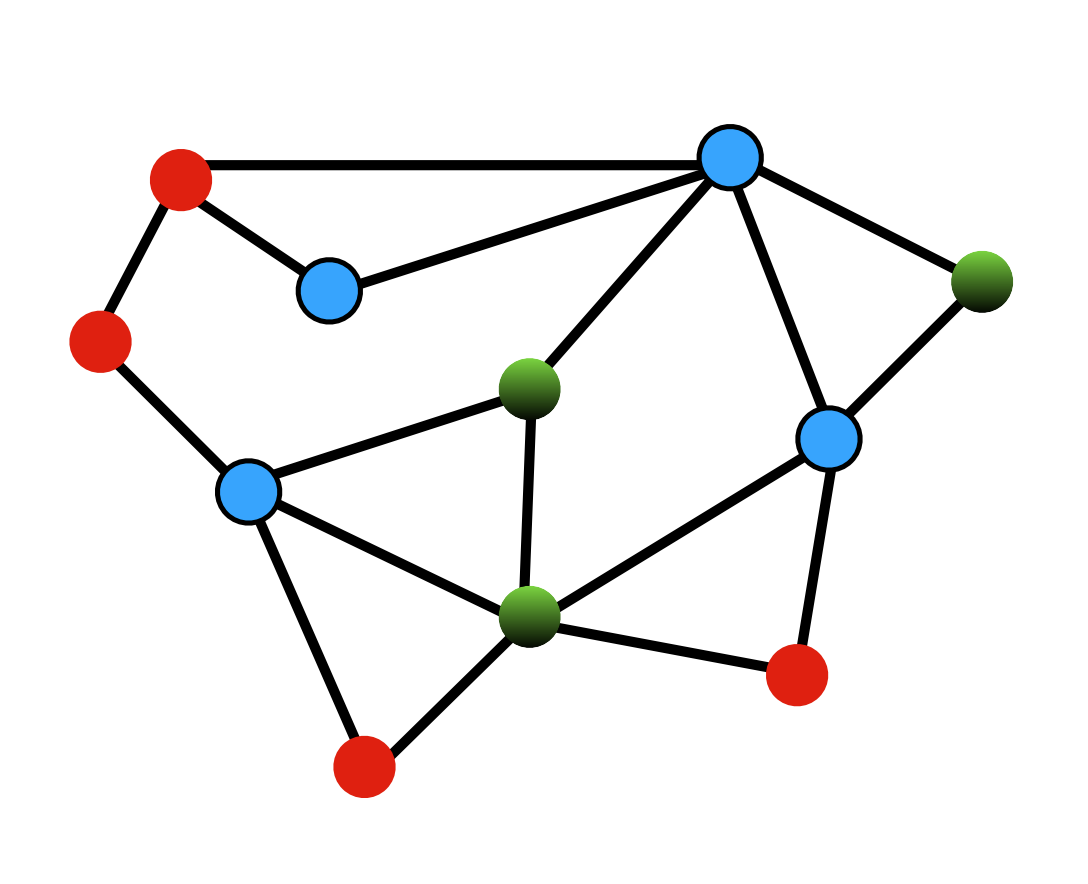
\includegraphics[scale=0.8]{media/sample-graph.png}
\caption{A sample graph}
\label{fig:sample-graph}
\end{figure}

\newpage
\bibliography{references}

\end{document}
